\section{Illustrative Example} \label{sec:expl}

We provide here a toy example to illustrate the upper bound approximation method and the lower bound feasibility and bound tightening procedures. 
For this example

$$A=
\left[
\scalebox{0.5}{%
	\begin{tabular}{ c c }
	$-1$ & $0$  \\ 
	$1$ & $0$  \\  
	$0$ & $-1$ \\
	$0$ & $1$  
	\end{tabular}%
} 
\right] \hspace*{0.25in} b=
\left[
\scalebox{0.5}{%
	\begin{tabular}{ c }
	$-0.5$  \\ 
	$3$ \\  
	$-0.5$ \\
	$3$  
	\end{tabular}%
} 
\right] \hspace*{0.25in} Q_1=
\left[
\scalebox{0.5}{%
	\begin{tabular}{ c c }
	$1$ & $0$  \\ 
	$0$ & $0$  
	\end{tabular}%
} 
\right] \hspace*{0.25in} Q_2=
\left[
\scalebox{0.5}{%
	\begin{tabular}{ c c }
	$0$ & $0$  \\ 
	$0$ & $1$  
	\end{tabular}%
} 
\right] \hspace*{0.25in} L=
\left[
\scalebox{0.5}{%
	\begin{tabular}{ c c }
	$1$ & $-3$  \\ 
	$2$ & $-1$  
	\end{tabular}%
} 
\right] \hspace*{0.25in} u^*=
\left[
\scalebox{0.5}{%
	\begin{tabular}{ c }
	$-2$  \\ 
	$4$   
	\end{tabular}%
} 
\right]
$$
which corresponds to the quadratic system 
$$F(\vx)=\left[\begin{array}{r} x_1^2+x_1-x_2 \\ x_2^2+2x_1-x_2 \end{array}\right]=\left[\begin{array}{r} -2 \\ 4 \end{array}\right] \hspace*{0.15in} \text{s.t.} \hspace*{0.15in} \Omega_{\vx}=\begin{array}{rcl} 0.5\leq & x_1 & \leq 3 \\ 0.5\leq & x_2 & \leq 3 \end{array} $$

Running the upper bound procedure produces an upper bound on the robustness margin of $2.63462$. Running the feasibility procedure results in an lower bound on the robustness margin of $1.20454$, while the bound tightening yields a lower bound of $1.706649$. 
 
Graphically we can see $F(\Omega_{\vx})$ with $\vu^*$ in \cref{fig:FOmega}.

\begin{figure}[htp!]
	\begin{center}
		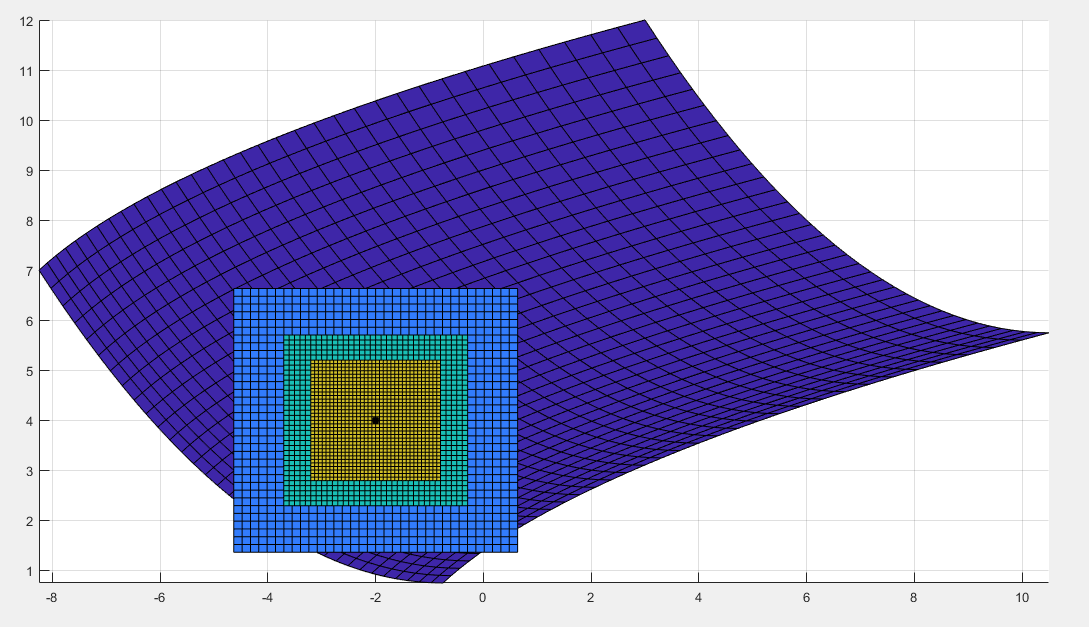
\includegraphics[scale=0.45]{Figures/newex} % {Figures/Rfeas}
	\end{center}
	\caption{Illustration of $F(\Omega_x)$ (dark blue surface), $u^*$ and $\Omega_{u^*}$ with radi given by the upper bound procedure (light blue box), bound tightening procedure (turquoise box), and feasibility procedure (yellow box).}
	\label{fig:FOmega}
\end{figure}

Notice that the bound tightening procedure produces a better approximation as theoretically predicted. All procedures were run using their most relaxed forms. 